\documentclass{standalone}
\usepackage{tikz}
\usetikzlibrary{automata,positioning}

\begin{document}
  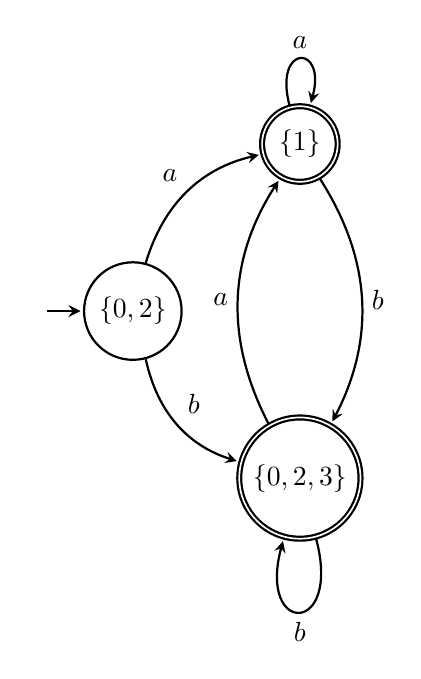
\begin{tikzpicture}[%
    >=stealth,
    shorten >=1pt,
    node distance=3cm,
    on grid,
    auto,
    state/.append style={minimum size=2em},
    thick
  ]
    \node[state, initial, initial text = {}] (A) {$\{0, 2\}$};
    \node[state] (B) [accepting, above right of=A] {$\{1\}$};
    \node[state] (C) [accepting, below right of=A] {$\{0, 2, 3\}$};

    \path[->] (A) +(-1,0) edge (A)
              (A)         edge [bend left]  node {$a$} (B)
              (A)         edge [bend right] node {$b$} (C)
              (B)         edge [loop above] node {$a$} (C)
              (C)         edge [loop below] node {$b$} (C)
              (C)         edge [bend left] node {$a$} (B)
              (B)         edge [bend left] node {$b$} (C);
  \end{tikzpicture}
\end{document}